\documentclass[12pt,oneside,reqno]{amsart}
\usepackage{mathtools, stackengine}
\numberwithin{equation}{section}
\usepackage{esint}
%\usepackage{undertilde}
\newcommand\norm[1]{\left\lVert#1\right\rVert}
\usepackage{tikz}
\usetikzlibrary{arrows} 
\usetikzlibrary{calc,angles,quotes}
\newtheorem{theorem}{Theorem}[section]
\newtheorem{remark}[theorem]{Remark}
\newtheorem{lemma}[theorem]{Lemma}
\newtheorem{corollary}[theorem]{Corollary}
\usepackage{caption}
\usepackage{subcaption}
\usepackage{longtable}
\usepackage{color,soul}
\usepackage{bm}
\usepackage{setspace}
\newcommand{\ba}{\backslash}
\usepackage{float}
\doublespacing
\usepackage{afterpage}
\usepackage{geometry} %may be sus
\usepackage[framed,numbered]{matlab-prettifier}
% turn "backspace" character (ASCII 8) into a tab (9) to avoid Matlab warning backspace
\catcode8=9
\lstset{
  style             = Matlab-editor,
  basicstyle        = {\ttfamily\tiny},
  mlshowsectionrules = true,
  upquote           = true
}

\newcommand{\spacer}{\vspace{6mm} \noindent}

\usepackage{enumitem}

% BIB stuff

%\usepackage{biblatex}
%\addbibresource{Matt_Bib.bib}

\usepackage{hyperref}


\begin{document}

\begin{enumerate}
    \item A standard Solow model with no technological change has the following features:
    \begin{enumerate}
        \item What is the function, g (kt), for $k_{t+1}$ = g ($k_t$): $\frac{(1-\delta)k_t+\sigma A_0 f(k_t)}{(1+n)}$ = $\frac{(.9)*k_t+0.15*10 *k_t^{0.4}}{(1.02)}$
        \item What is the stable steady state level of capital per worker? \\
        $ $, lets solve for $k_t$ \\
        $k_t*(1.02) = 0.9*k_t+1.5*k_t^{0.4}$\\
        $0.12k_t=1.5*k_t^{0.4}$\\
        $0.12k_t^{0.6}=1.5$\\
        $k_t=(\frac{1.5}{0.12})^{\frac{1}{0.6}}=67.32608$
        
        \item Is the economy maximizing steady state consumption per worker? If not, what savings rate and what level of steady state capital per worker would maximize steady state consumption per worker?\\
        to maximize steady state consumption per worker solve\\ $\max_{\Bar{k}} \Bar{A}f(\Bar{k})-(\delta+n)\Bar{k}$, by taking a derivitive\\
        $\Bar{A}f'(\Bar{k})=\delta+n$\\
        $10*.4*\Bar{k}^{-0.6}=.12$\\
        $=345.248$\\
        Solving for the saving rate\\
        $(\delta+n)k^*=\sigma\Bar{A}f(k^*)$\\
        $\sigma = \frac{(.1+.02)*345.248}{10*(345.248)^{0.4}}$\\
        $=0.4$ 
        %using the new savings rate the optimal capital per worker is\\
        %$\frac{(.9)*k_t+0.4*10 *k_t^{0.4}}{(1.02)}= 345.248$\\
        The Capital per work of 345.248 and a savings rate of .4 will maximize the consumption
    \end{enumerate}
    \item The economy in question 1 is at the steady state for 10 periods. In the eleventh period, the savings rate increases to 30\% and remains there. Simulate the economy for 100 periods (10 before the change, 90 with the new savings rate). Plot capital per worker, output per worker and consumption per worker on separate graphs for those 100 periods. Include the figure in the pdf. What do you notice in the figure?
    \begin{figure}[h]
        \centering
        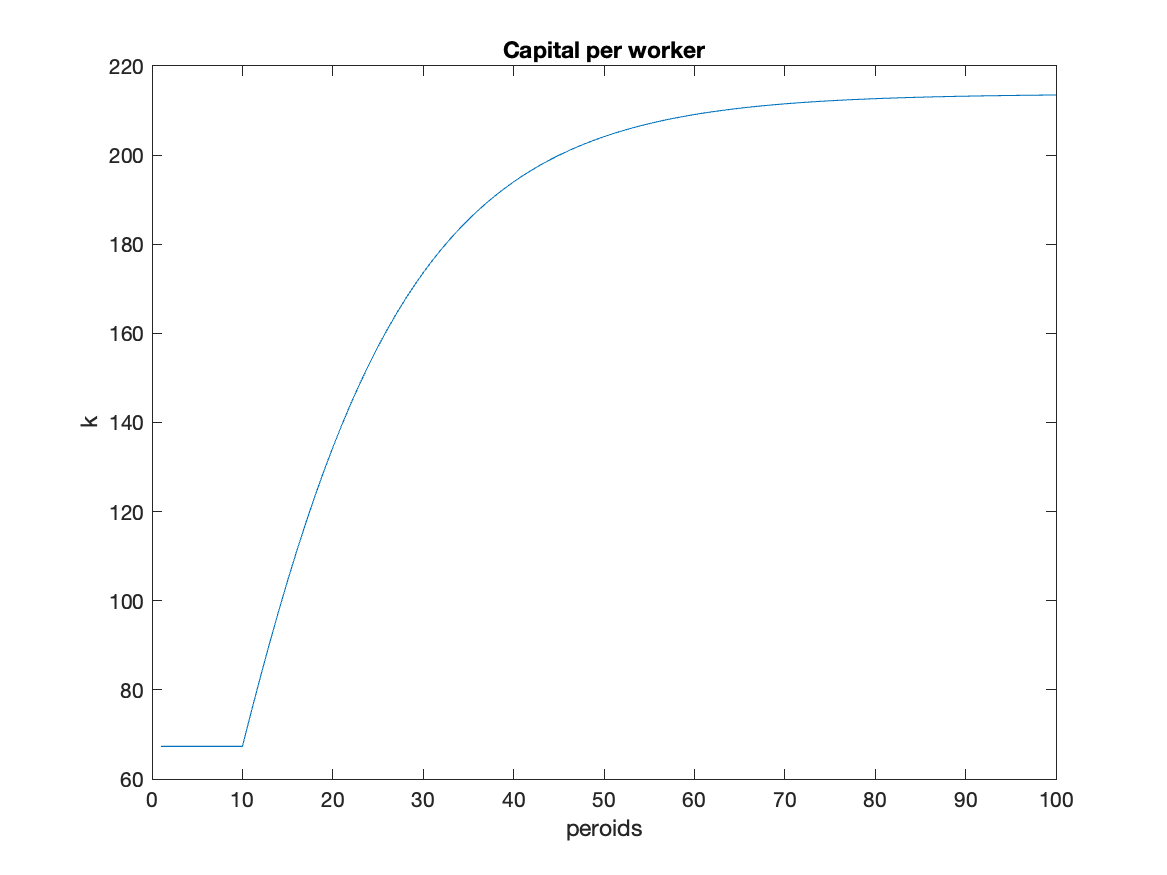
\includegraphics[width =.5\linewidth]{HW1/HW1_Q2_a.png}
        \caption{Capital per Worker}
    \end{figure}
    \vspace{-.5cm}
    \begin{figure}[h]
        \centering
        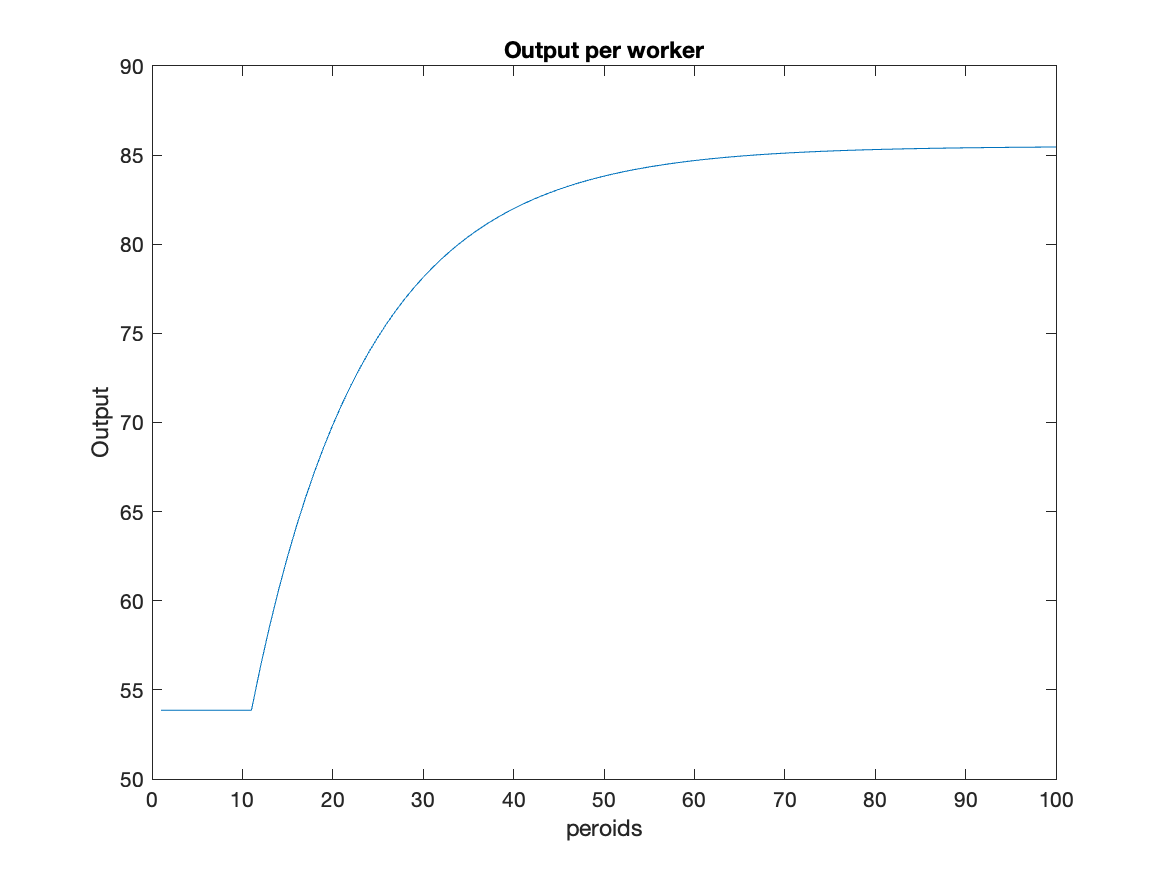
\includegraphics[width =.5\linewidth]{HW1/HW1_Q2_b.png}
        \caption{Output per Worker}
    \end{figure}
    \begin{figure}[h]
        \centering
        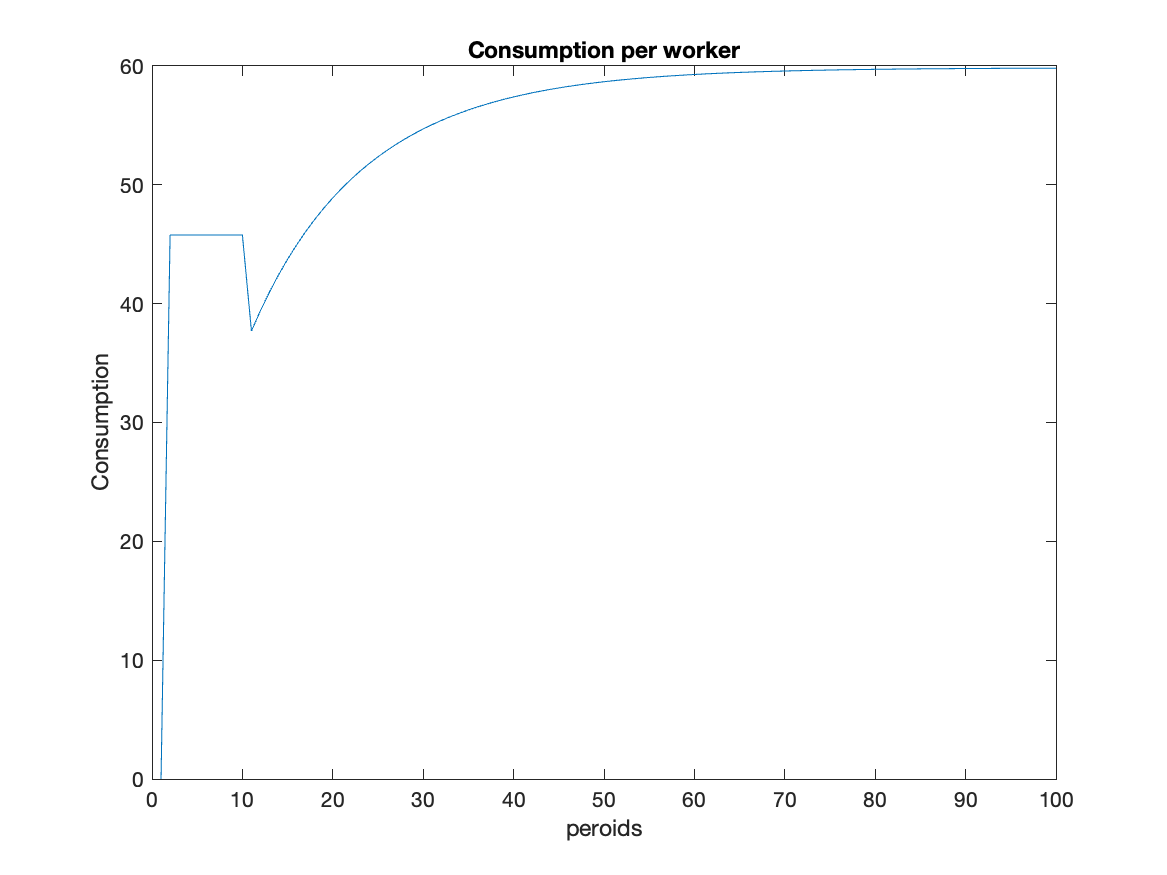
\includegraphics[width =.5\linewidth]{HW1/HW1_Q2_c.png}
        \caption{Consumption per Worker}
    \end{figure}
\item A stochastic Solow model has the following features
\begin{enumerate}
    \item What is the stable steady state level of capital per worker?
    we will first  calculate the steady state assuming that $z_{t}$ is zero so we will solve $\frac{(1-\delta)k_t+\sigma A_0 f(k_t)}{(1+n)} = k = \frac{(.975)*k_t+(0.1*5)*k^{0.4}}{(1.01)}= 84.1078$
    \item it is not explicitly listed but we will use a random normal with a $\sigma =1 \text{ and } \mu =0$ and $z_0 =e^{\sim N(0,1)}$
\end{enumerate}
\end{enumerate}



\end{document}